\section{Convergence: Integrating External Agent Frameworks}\label{sec:convergence}

The preceding sections develop Operon's structural analysis, epistemic topology,
and formal verification foundations. This section summarizes how these tools
extend to external agent orchestration systems through a typed adapter
architecture. A standalone companion paper provides the full treatment, including
implementation details, all 107 examples, and complete TLA+ specification
listings; this section is self-contained but deliberately concise.

\begin{center}
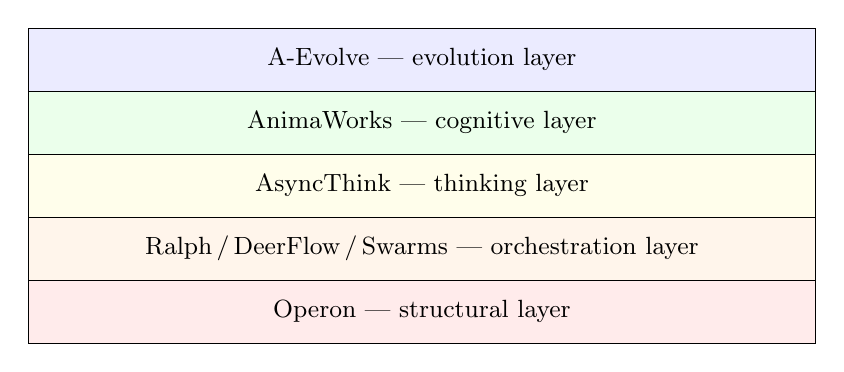
\begin{tikzpicture}[
  layer/.style={draw, minimum width=10cm, minimum height=0.8cm, font=\small},
  >=latex
]
\node[layer, fill=blue!8]  (L5) at (0,3.2) {A-Evolve --- evolution layer};
\node[layer, fill=green!8] (L4) at (0,2.4) {AnimaWorks --- cognitive layer};
\node[layer, fill=yellow!8](L3) at (0,1.6) {AsyncThink --- thinking layer};
\node[layer, fill=orange!8](L2) at (0,0.8) {Ralph\,/\,DeerFlow\,/\,Swarms --- orchestration layer};
\node[layer, fill=red!8]   (L1) at (0,0.0) {Operon --- structural layer};
\end{tikzpicture}
\end{center}

Every adapter produces an \texttt{ExternalTopology}---a framework-agnostic
intermediate representation carrying a source tag, a pattern name, agent
specifications, directed communication edges, and arbitrary metadata. The
analysis pipeline is source-agnostic: \texttt{analyze\_external\_topology()}
consumes any \texttt{ExternalTopology} and applies three of the four epistemic
bounds---error amplification, sequential penalty, and tool density---plus a
topology-mismatch flag to produce topology advice, structural warnings, and
a composite risk score. (Parallel acceleration is computed by the epistemic
layer but not included in the adapter risk score.) Adding a new orchestration target therefore requires
writing a single parse function---no changes to the analysis code.

Four TLA+ specifications verify safety invariants that are difficult to test
exhaustively at the unit level: \emph{TemplateExchangeProtocol} (provenance and
trust monotonicity), \emph{DevelopmentalGating} (irreversible stage transitions
and capability constraints), \emph{ConvergenceDetection} (intervention-count
convergence or HALT), and \emph{EvolutionGating} (monotonic score safety for
A-Evolve's evolutionary loop). Together, these cover the critical safety
boundaries of the convergence stack.

For the complete treatment---including adapter implementation details, template
exchange protocols, memory bridge semantics, TLA+ specification listings, and all
107 worked examples---see the standalone convergence companion
paper.\footnote{\url{https://coredipper.github.io/operon/convergence/}}

A live evaluation harness (Example~107) measures quality, latency, and token
cost across Gemini~API, Claude~CLI, and Codex~CLI providers. Guided
multi-stage pipelines show a consistent $+6.2\%$ quality improvement over
unguided configurations; single-agent CLI execution shows no effect,
confirming that structural guidance helps when there is topology to guide.
